% This LaTeX was auto-generated from MATLAB code.
% To make changes, update the MATLAB code and export to LaTeX again.

\documentclass{article}

\usepackage[utf8]{inputenc}
\usepackage[T1]{fontenc}
\usepackage{lmodern}
\usepackage{graphicx}
\usepackage{color}
\usepackage{listings}
\usepackage{hyperref}
\usepackage{amsmath}
\usepackage{amsfonts}
\usepackage{epstopdf}
\usepackage{matlab}

\sloppy
\epstopdfsetup{outdir=./}
\graphicspath{ {./ejercicio10_images/} }

\matlabmultipletitles

\begin{document}

\matlabtitle{Ejercicio N°10}

\begin{matlabcode}
clc;
clear;
\end{matlabcode}

\begin{par}
\begin{flushleft}
Se definen simbólicas las variables
\end{flushleft}
\end{par}

\begin{matlabcode}
syms t vc1(t) vc2(t) il1(t) il2(t) L1 L2 K1 K2;
\end{matlabcode}

\begin{par}
\begin{flushleft}
Se plantean las ecuaciones y se obtienen las matrices de la forma generalizada
\end{flushleft}
\end{par}

\begin{matlabcode}
M=[-K1 0 0 0;0 K2 0 0;0 0 L1 L2;0 0 0 -L2]
\end{matlabcode}
\begin{matlabsymbolicoutput}
M = 
    $\displaystyle \left(\begin{array}{cccc}
-K_1  & 0 & 0 & 0\\
0 & K_2  & 0 & 0\\
0 & 0 & L_1  & L_2 \\
0 & 0 & 0 & -L_2 
\end{array}\right)$
\end{matlabsymbolicoutput}
\begin{matlabcode}
N=[0 0 1 0; 0 0 -1 1;1 0 0 0;0 1 0 0]
\end{matlabcode}
\begin{matlaboutput}
N = 4x4    
     0     0     1     0
     0     0    -1     1
     1     0     0     0
     0     1     0     0

\end{matlaboutput}
\begin{matlabcode}
u=[0;0;0;0]
\end{matlabcode}
\begin{matlaboutput}
u = 4x1    
     0
     0
     0
     0

\end{matlaboutput}

\begin{par}
\begin{flushleft}
Se expresan las matrices de la forma normalizada
\end{flushleft}
\end{par}

\begin{matlabcode}
A=-1.*(M\N)
\end{matlabcode}
\begin{matlabsymbolicoutput}
A = 
    $\displaystyle \left(\begin{array}{cccc}
0 & 0 & \frac{1}{K_1 } & 0\\
0 & 0 & \frac{1}{K_2 } & -\frac{1}{K_2 }\\
-\frac{1}{L_1 } & -\frac{1}{L_1 } & 0 & 0\\
0 & \frac{1}{L_2 } & 0 & 0
\end{array}\right)$
\end{matlabsymbolicoutput}

\begin{par}
\begin{flushleft}
Se definen las variables de estado
\end{flushleft}
\end{par}

\begin{matlabcode}
x=[vc1;vc2;il1;il2]
\end{matlabcode}
\begin{matlabsymbolicoutput}
x(t) = 
    $\displaystyle \left(\begin{array}{c}
{\textrm{vc}}_1 \left(t\right)\\
{\textrm{vc}}_2 \left(t\right)\\
{\textrm{il}}_1 \left(t\right)\\
{\textrm{il}}_2 \left(t\right)
\end{array}\right)$
\end{matlabsymbolicoutput}

\begin{par}
\begin{flushleft}
Expresando el sistema en forma diferencial
\end{flushleft}
\end{par}

\begin{matlabcode}
odes = diff(x) == A*x
\end{matlabcode}
\begin{matlabsymbolicoutput}
odes(t) = 
    $\displaystyle \left(\begin{array}{c}
\frac{\partial }{\partial t}\;{\textrm{vc}}_1 \left(t\right)=\frac{{\textrm{il}}_1 \left(t\right)}{K_1 }\\
\frac{\partial }{\partial t}\;{\textrm{vc}}_2 \left(t\right)=\frac{{\textrm{il}}_1 \left(t\right)}{K_2 }-\frac{{\textrm{il}}_2 \left(t\right)}{K_2 }\\
\frac{\partial }{\partial t}\;{\textrm{il}}_1 \left(t\right)=-\frac{{\textrm{vc}}_1 \left(t\right)}{L_1 }-\frac{{\textrm{vc}}_2 \left(t\right)}{L_1 }\\
\frac{\partial }{\partial t}\;{\textrm{il}}_2 \left(t\right)=\frac{{\textrm{vc}}_2 \left(t\right)}{L_2 }
\end{array}\right)$
\end{matlabsymbolicoutput}

\begin{par}
\begin{flushleft}
Reemplazando los valores de los componentes
\end{flushleft}
\end{par}

\begin{matlabcode}
clear K1 K2 L1 L2;
syms C1 C2 C3 C4;
K1=1/25;K2=1/72;L1=1;L2=18;
A=subs(A);
\end{matlabcode}

\begin{par}
\begin{flushleft}
Las ecuaciones diferenciales son
\end{flushleft}
\end{par}

\begin{matlabcode}
odes = diff(x) == A*x;
\end{matlabcode}

\begin{par}
\begin{flushleft}
Definiendo las condiciones iniciales y tiempo de simulacion
\end{flushleft}
\end{par}

\begin{matlabcode}
vc01=1;
vc02=0;
il01=0;
il02=0;
ti=0;
tf=10;
Xant=[vc01;vc02;il01;il02];
constantes=x(0)==Xant;
[il1Sol(t), il2Sol(t), vc1Sol(t), vc2Sol(t)] = dsolve(odes,constantes);
\end{matlabcode}


\matlabtitle{Tensión en C1}

\begin{matlabcode}
vc1Sol
\end{matlabcode}
\begin{matlabsymbolicoutput}
vc1Sol(t) = 
    $\displaystyle \frac{8 \cos \left(10 t\right)}{33}+\frac{25 \cos \left(t\right)}{33}$
\end{matlabsymbolicoutput}

\matlabtitle{Tensión en C2}

\begin{matlabcode}
vc2Sol
\end{matlabcode}
\begin{matlabsymbolicoutput}
vc2Sol(t) = 
    $\displaystyle \frac{8 \cos \left(10 t\right)}{11}-\frac{8 \cos \left(t\right)}{11}$
\end{matlabsymbolicoutput}

\matlabtitle{Corriente en L1}

\begin{matlabcode}
il1Sol
\end{matlabcode}
\begin{matlabsymbolicoutput}
il1Sol(t) = 
    $\displaystyle -\frac{16 \sin \left(10 t\right)}{165}-\frac{\sin \left(t\right)}{33}$
\end{matlabsymbolicoutput}

\matlabtitle{Corriente en L2}

\begin{matlabcode}
il2Sol
\end{matlabcode}
\begin{matlabsymbolicoutput}
il2Sol(t) = 
    $\displaystyle \frac{2 \sin \left(10 t\right)}{495}-\frac{4 \sin \left(t\right)}{99}$
\end{matlabsymbolicoutput}


\vspace{1em}

\begin{matlabcode}
fplot(il1Sol,vc1Sol,[ti,tf])
title('Phase Portrait')
xlabel('iL1[A]')
ylabel('VC1 [V]')
\end{matlabcode}
\begin{center}
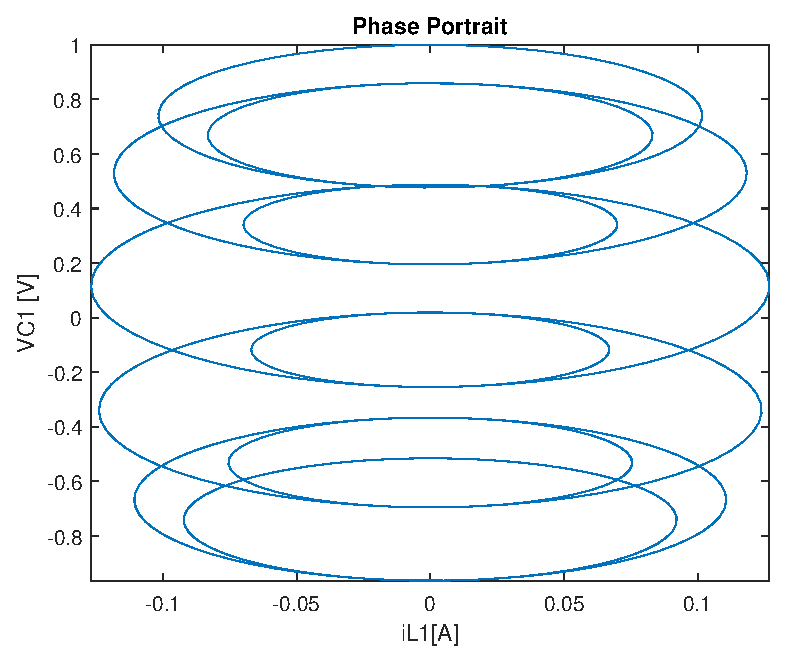
\includegraphics[width=\maxwidth{56.196688409433015em}]{figure_0_10}
\end{center}


\begin{matlabcode}
fplot(il1Sol,vc2Sol,[ti,tf])
title('Phase Portrait')
xlabel('iL1[A]')
ylabel('VC2 [V]')
\end{matlabcode}
\begin{center}
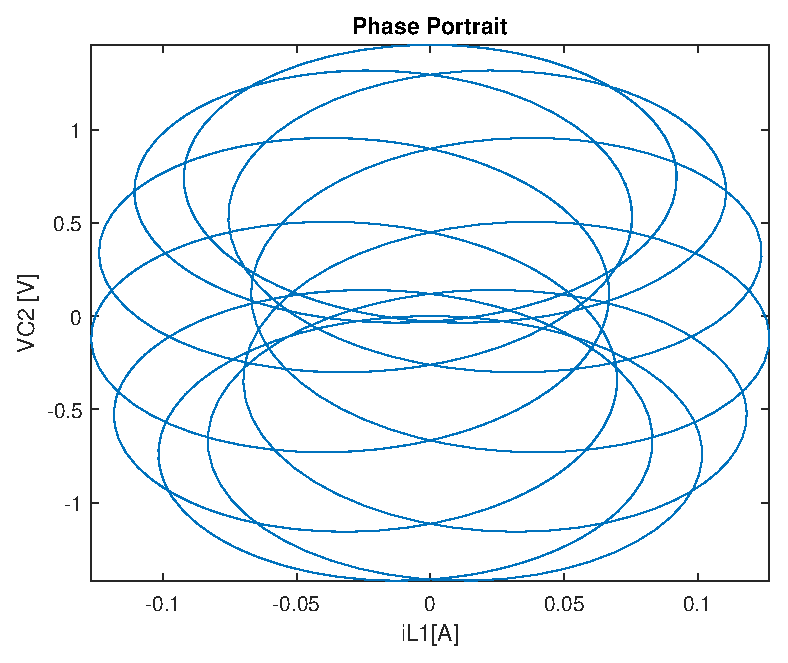
\includegraphics[width=\maxwidth{56.196688409433015em}]{figure_1_10}
\end{center}


\begin{matlabcode}
fplot(il2Sol,vc1Sol,[ti,tf])
title('Phase Portrait')
xlabel('iL2[A]')
ylabel('VC1 [V]')
\end{matlabcode}
\begin{center}
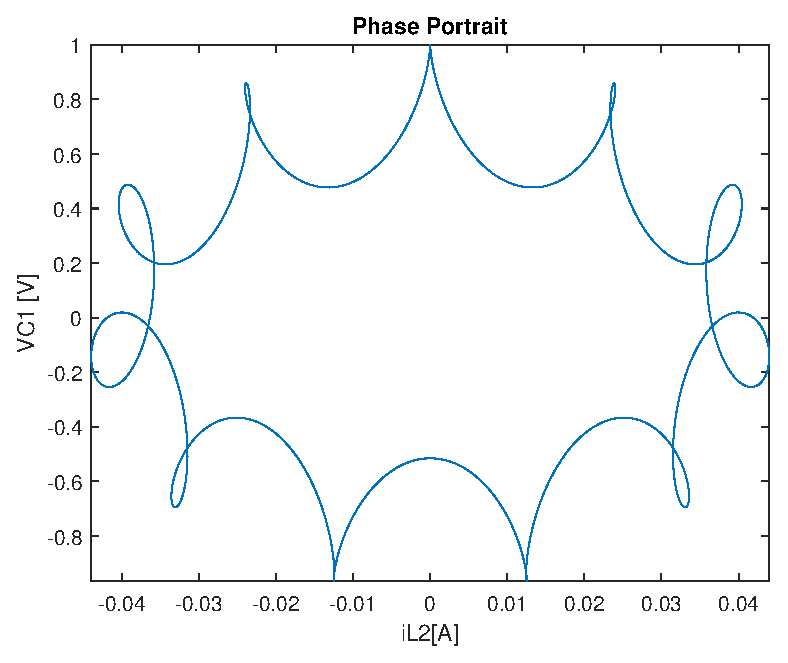
\includegraphics[width=\maxwidth{56.196688409433015em}]{figure_2_10}
\end{center}


\begin{matlabcode}
fplot(il2Sol,vc2Sol,[ti,tf])
title('Phase Portrait')
xlabel('iL2[A]')
ylabel('VC2 [V]')
\end{matlabcode}
\begin{center}
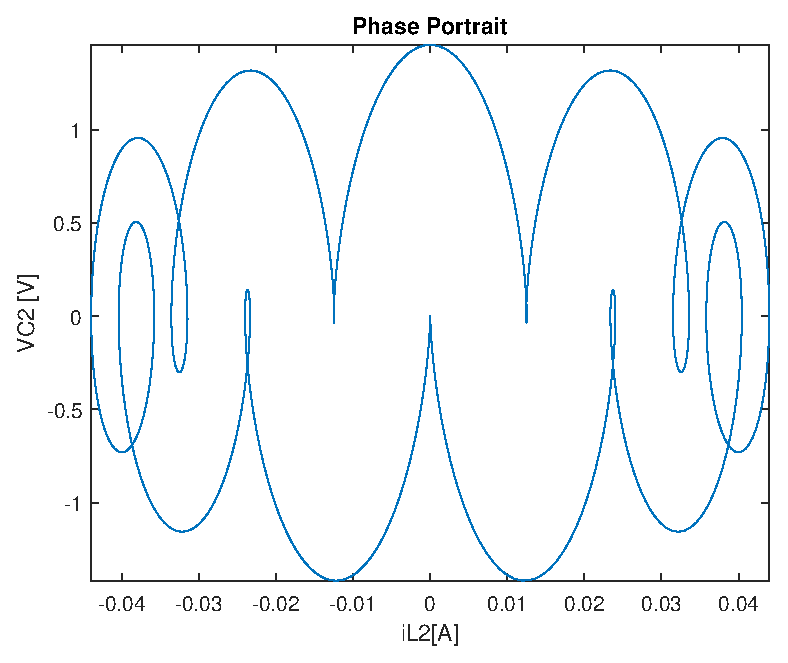
\includegraphics[width=\maxwidth{56.196688409433015em}]{figure_3_10}
\end{center}

\end{document}
